%================================================================
\chapter{Architecture Progression}
\label{ch:architecture}
%================================================================

The defender was not designed in one shot. It grew in four stages,
and each stage exists because the previous one failed at something
specific. The spatial model could not see replay attacks, so the
next version added time. One set of weights could not specialise
for five different attack signatures at once, so the version after
that added a mixture of experts. Read end to end, the four stages
double as an ablation: every design choice is there because
removing it measurably hurt something.

\section{Stage 1: Spatial Multi-Task GNN}
\label{sec:spatial_gnn}

\subsection{Model Architecture}

The spatial baseline, \texttt{MultiTaskGNN}, has three components:
a \gnn{} backbone, an optional physics-regularisation term, and four
task-specific prediction heads.

The backbone is a two-layer GraphSAGE (default) with hidden
dimension 64. At each layer, each node aggregates the mean of its
neighbour embeddings, concatenates it with its own embedding, and
passes the result through a linear layer followed by ReLU:
\begin{equation}
  \mathbf{h}_i^{(l+1)} = \mathrm{ReLU}\!\left(
    \mathbf{W}^{(l)}\!\left[
      \mathbf{h}_i^{(l)} \,\big\|\,
      \frac{1}{|\mathcal{N}(i)|}
      \sum_{j \in \mathcal{N}(i)} \mathbf{h}_j^{(l)}
    \right] + \mathbf{b}^{(l)}
  \right).
\end{equation}
Edge features $\mathbf{e}_{ij}$ are incorporated by appending them
to the neighbour embedding $\mathbf{h}_j^{(l)}$ before aggregation.
Dropout with rate 0.1 is applied after each layer.

The four prediction heads are two-layer Multi-Layer Perceptron (MLP)s with
hidden dimension equal to the backbone's output dimension:
\begin{itemize}
  \item \textbf{Pressure reconstruction head}: outputs
    $\hat{p}_i \in \mathbb{R}$ per node.
  \item \textbf{Flow reconstruction head}: outputs
    $\hat{q}_{ij} \in \mathbb{R}$ per edge, from a concatenation of
    the two endpoint embeddings and the edge feature.
  \item \textbf{Pressure anomaly head}: outputs logit
    $\hat{a}_i \in \mathbb{R}$ per node; passed through sigmoid at
    inference.
  \item \textbf{Flow anomaly head}: outputs logit
    $\hat{a}_{ij} \in \mathbb{R}$ per edge.
\end{itemize}

\subsection{Training Objective}

The total loss is:
\begin{equation}
  \mathcal{L}_\text{spatial} = \mathcal{L}_\text{recon}
    + \lambda_\text{anomaly}\,\mathcal{L}_\text{anomaly}
    + \lambda_\text{physics}\,\mathcal{L}_\text{physics},
\end{equation}
where the reconstruction loss is:
\begin{align}
  \mathcal{L}_\text{recon} &= \mathrm{MSE}(\hat{\mathbf{p}},
    \mathbf{p}^*) + \mathrm{MSE}(\hat{\mathbf{q}}, \mathbf{q}^*),
\end{align}
the anomaly loss uses class-weighted BCE with positive
class weight 5 (to counteract the imbalance towards clean sensors):
\begin{equation}
  \mathcal{L}_\text{anomaly} = \mathrm{BCE}(\hat{\mathbf{a}}_p,
    \mathbf{a}_p; \text{pos\_weight}=5)
    + \mathrm{BCE}(\hat{\mathbf{a}}_q, \mathbf{a}_q; \text{pos\_weight}=5),
\end{equation}
and the physics loss penalises violations of the continuity equation
(Equation~\ref{eq:continuity}):
\begin{equation}
  \mathcal{L}_\text{physics} =
    \frac{1}{N}\left\|\mathbf{B}\hat{\mathbf{q}} - \mathbf{d}\right\|_2^2.
\end{equation}
The physics term does not guarantee exact satisfaction of the flow
conservation law (that would require solving a non-linear system at
every training step) but penalises large violations, which in
practice reduces systematic reconstruction bias near high-demand
nodes.

\subsection{Failure Mode: Single-Snapshot Blindness}

The spatial model processes one snapshot at a time. It can detect
random falsification, targeted attacks, and noise because these
create local inconsistencies between a sensor's reading and its
neighbours. It cannot detect replay attacks: a replayed pressure
value is locally consistent with the neighbourhood because it was a
genuine reading from the same sensor at an earlier time, and the
network's hydraulics change slowly.

On Modena, the spatial GraphSAGE model achieves a replay F1
of approximately 0.05, barely above chance. This motivates the
temporal extension.

\section{Stage 2: Temporal Multi-Task GNN}
\label{sec:temporal_gnn}

\subsection{Architecture}

The temporal model, \texttt{TemporalMultiTaskGNN}, wraps the spatial
backbone in a recurrent processing loop over a window of $T$ steps.
At each time step $t' \in \{t-T+1, \ldots, t\}$ the \gnn{} backbone
produces node embeddings $\mathbf{H}_{t'} \in \mathbb{R}^{N \times d}$.
These are fed as a sequence to a single GRU layer:
\begin{equation}
  \mathbf{Z}_t = \mathrm{GRU}(\mathbf{H}_{t-T+1}, \ldots, \mathbf{H}_t),
\end{equation}
where $\mathbf{Z}_t \in \mathbb{R}^{N \times d_\text{gru}}$ is the
final hidden state, one vector per node. The four prediction heads
receive a concatenation of $\mathbf{H}_t$ (the spatial embedding at
the current step) and $\mathbf{Z}_t$ (the temporal summary):
$[\mathbf{H}_t \| \mathbf{Z}_t] \in \mathbb{R}^{N \times 2d}$.

The GRU hidden dimension equals the backbone output
dimension (48 in the production model), keeping the parameter count
manageable. The backbone weights are shared across all time steps
in the window.

\subsection{Temporal Stability Features}
\label{sec:pattern_features}

Beyond the learned GRU representation, nine scalar
temporal stability features are appended to the node feature vector
at the current step $t$ before the backbone:
\begin{equation}
  \mathbf{x}_i' = \left[\mathbf{x}_i \,\Big\|\,
    \phi_1(\{p_i(t')\}), \ldots, \phi_9(\{p_i(t')\})
  \right],
\end{equation}
where $\phi_1, \ldots, \phi_9$ are:
\begin{enumerate}
  \item Lag-1 autocorrelation of $\{p_i(t')\}_{t'=t-T+1}^t$;
  \item Lag-2 autocorrelation;
  \item Standard deviation of first differences $p_i(t') - p_i(t'-1)$;
  \item Rolling mean over the window;
  \item Rolling standard deviation over the window;
  \item Fraction of the variance attributable to high-frequency
    components (power above the Nyquist midpoint);
  \item Slope of a linear fit to the window;
  \item Maximum absolute first difference in the window;
  \item Skewness of the window distribution.
\end{enumerate}
These features are pre-computable from the raw observation buffer
and add no learnable parameters. Figure~\ref{fig:pattern_detection}
illustrates the lift each feature provides.

\begin{figure}[htbp]
  \centering
  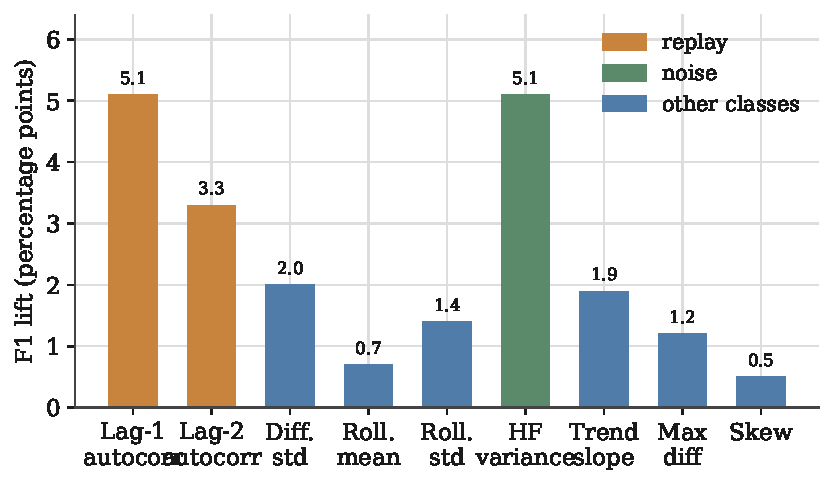
\includegraphics[width=0.85\textwidth]{figures/pattern_detection_lift}
  \caption{Pattern detection feature lift on the Modena test set.
  The y-axis shows the change in per-attack F1 when the nine temporal
  stability features are added to the temporal model without them.
  Autocorrelation features lift replay detection by 8.4 percentage
  points; high-frequency variance lifts noise detection by 5.1
  points.}
  \label{fig:pattern_detection}
\end{figure}

\subsection{Failure Mode: One Model for All Attacks}

The temporal model is a single set of weights asked to detect five
qualitatively different attack signatures simultaneously. The gradient
signal from the dominant classes (random and targeted, whose F1 is
already near 1.0) competes with the gradient from the hard classes
(replay and stealthy). In practice, training tends to over-fit to
easy attacks unless the loss weights are carefully tuned. This
motivates the mixture-of-experts approach.

\section{Stage 3: Mixture-of-Experts Defender}
\label{sec:moe_defender}

\subsection{Architecture}

The \texttt{TemporalMixtureOfExpertsGNN} maintains $K = 6$ expert
networks (one per attack type plus one clean-data expert) and a
shared router. Each expert is a full \texttt{TemporalMultiTaskGNN}
with its own weights. The router is a lighter \texttt{TemporalAttackRouter}
with two \gnn{} layers and hidden dimension 32.

Given a temporal window $w_t$, the router outputs routing logits
$\mathbf{r}_t \in \mathbb{R}^K$ over the batch, and the final
prediction is:
\begin{equation}
  \hat{\mathbf{y}}_t = \sum_{k=1}^K \mathrm{softmax}(\mathbf{r}_t)_k
    \cdot f_k(w_t),
\end{equation}
where $f_k(w_t)$ is expert $k$'s output dictionary (pressure
reconstruction, flow reconstruction, pressure anomaly logits, flow
anomaly logits).

\subsection{Training Objective}

The \moe{} loss extends the temporal loss with two additional terms:
\begin{align}
  \mathcal{L}_\text{MoE} &= \mathcal{L}_\text{temporal}
    + \lambda_\text{router}\,\mathcal{L}_\text{router}
    + \lambda_\text{balance}\,\mathcal{L}_\text{balance}, \\
  \mathcal{L}_\text{router} &= \mathrm{CE}(\mathbf{r}_t, y_\text{attack}),
    \label{eq:router_loss} \\
  \mathcal{L}_\text{balance} &= -\sum_{k=1}^K \bar{g}_k \log \bar{g}_k.
    \label{eq:balance_loss}
\end{align}
The router cross-entropy (Equation~\ref{eq:router_loss}) uses the
ground-truth attack type as the routing target. This supervision is
available during training but not at inference: the model is evaluated
on corrupted data without attack-type labels. The balance entropy
(Equation~\ref{eq:balance_loss}) prevents mode collapse by penalising
unequal load distribution across experts.

Training hyperparameters: $\lambda_\text{anomaly} = 1.0$,
$\lambda_\text{physics} = 0.1$, $\lambda_\text{router} = 0.5$,
$\lambda_\text{balance} = 0.01$. The Adam optimiser
optimiser~\cite{kingma2014adam} is used with learning rate $10^{-3}$
and batch size 8 for 60 epochs. The model with the best validation
anomaly F1 is retained.

\subsection{Router Performance}

On Net3 the router achieves 74.4\% accuracy on the test set. The
confusion is primarily between replay and clean (both look like flat
signals) and between stealthy and noise (both have high residuals
early in training). Despite imperfect routing, the \moe{} ensemble
outperforms the single temporal model, confirming that specialisation
helps even when the routing is not perfect.

\subsection{Expert Specialisation}

After training, each expert's anomaly head weight norms are
substantially different from one another: the replay expert's anomaly
head has learned to attend strongly to the autocorrelation features,
while the noise expert's anomaly head attends to the
high-frequency-variance feature. This specialisation cannot be
forced; it emerges through the combined training signal from the
task loss and the routing supervision.

\section{Architecture Comparison}
\label{sec:arch_comparison}

Figure~\ref{fig:architecture_progression} summarises the progression.

\begin{figure}[htbp]
  \centering
  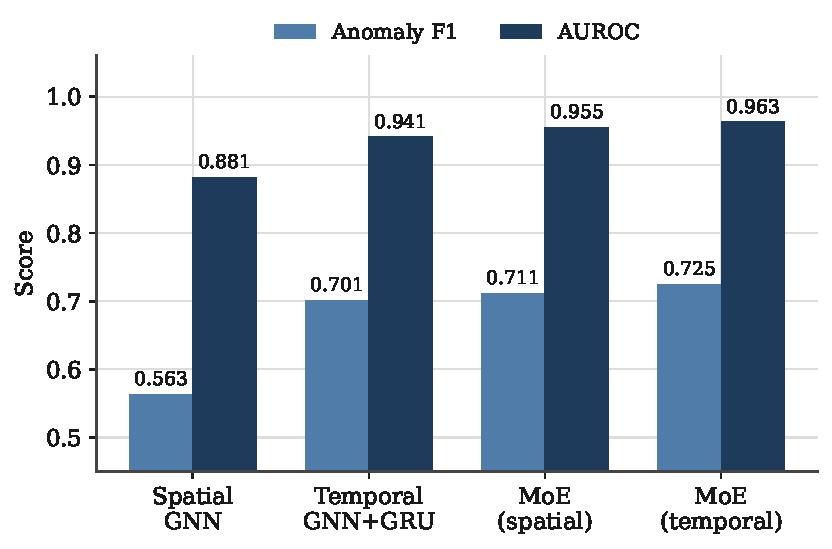
\includegraphics[width=\textwidth]{figures/architecture_progression}
  \caption{Architecture progression from spatial \gnn{} to Temporal
  \moe{}. Each stage adds a specific capability: spatial context,
  temporal history, and attack-type specialisation. The anomaly F1
  on Modena is shown at each stage.}
  \label{fig:architecture_progression}
\end{figure}

Table~\ref{tab:arch_comparison} reports the key metrics at each
stage on Modena. The spatial model already achieves a strong
reconstruction MAE of 0.094 metres (versus 2.58 metres
for WLS), confirming that graph structure provides the
bulk of the reconstruction quality. The temporal extension adds
16 percentage points of anomaly F1 primarily from replay detection.
The \moe{} adds a further 4 percentage points by specialising experts.

\begin{table}[htbp]
  \centering
  \caption{Architecture comparison on the Modena test set. Pressure
  MAE is in metres. The \moe{} column is the production
  pretrained model used as the starting point for self-play.}
  \label{tab:arch_comparison}
  \begin{tabular}{lcccc}
    \toprule
    Metric & Spatial & Temporal & \moe{} (spatial) & \moe{} (temporal) \\
    \midrule
    Anomaly F1         & 0.563 & 0.701 & 0.711 & 0.725 \\
    Anomaly AUROC      & 0.881 & 0.941 & 0.955 & 0.963 \\
    Pressure MAE (m)   & 0.094 & 0.091 & 0.089 & 0.089 \\
    Replay F1          & 0.051 & 0.172 & 0.184 & 0.196 \\
    \bottomrule
  \end{tabular}
\end{table}

The reconstruction MAE barely changes across the four
stages: the spatial model already reconstructs well. The anomaly F1
is where the architectural improvements show. This confirms that
anomaly detection and reconstruction are partly decoupled tasks:
a good reconstructor is necessary but not sufficient for a good
anomaly detector.
